\documentclass{standalone}
\usepackage{pgfplots}
\pgfplotsset{compat=newest}

\begin{document}
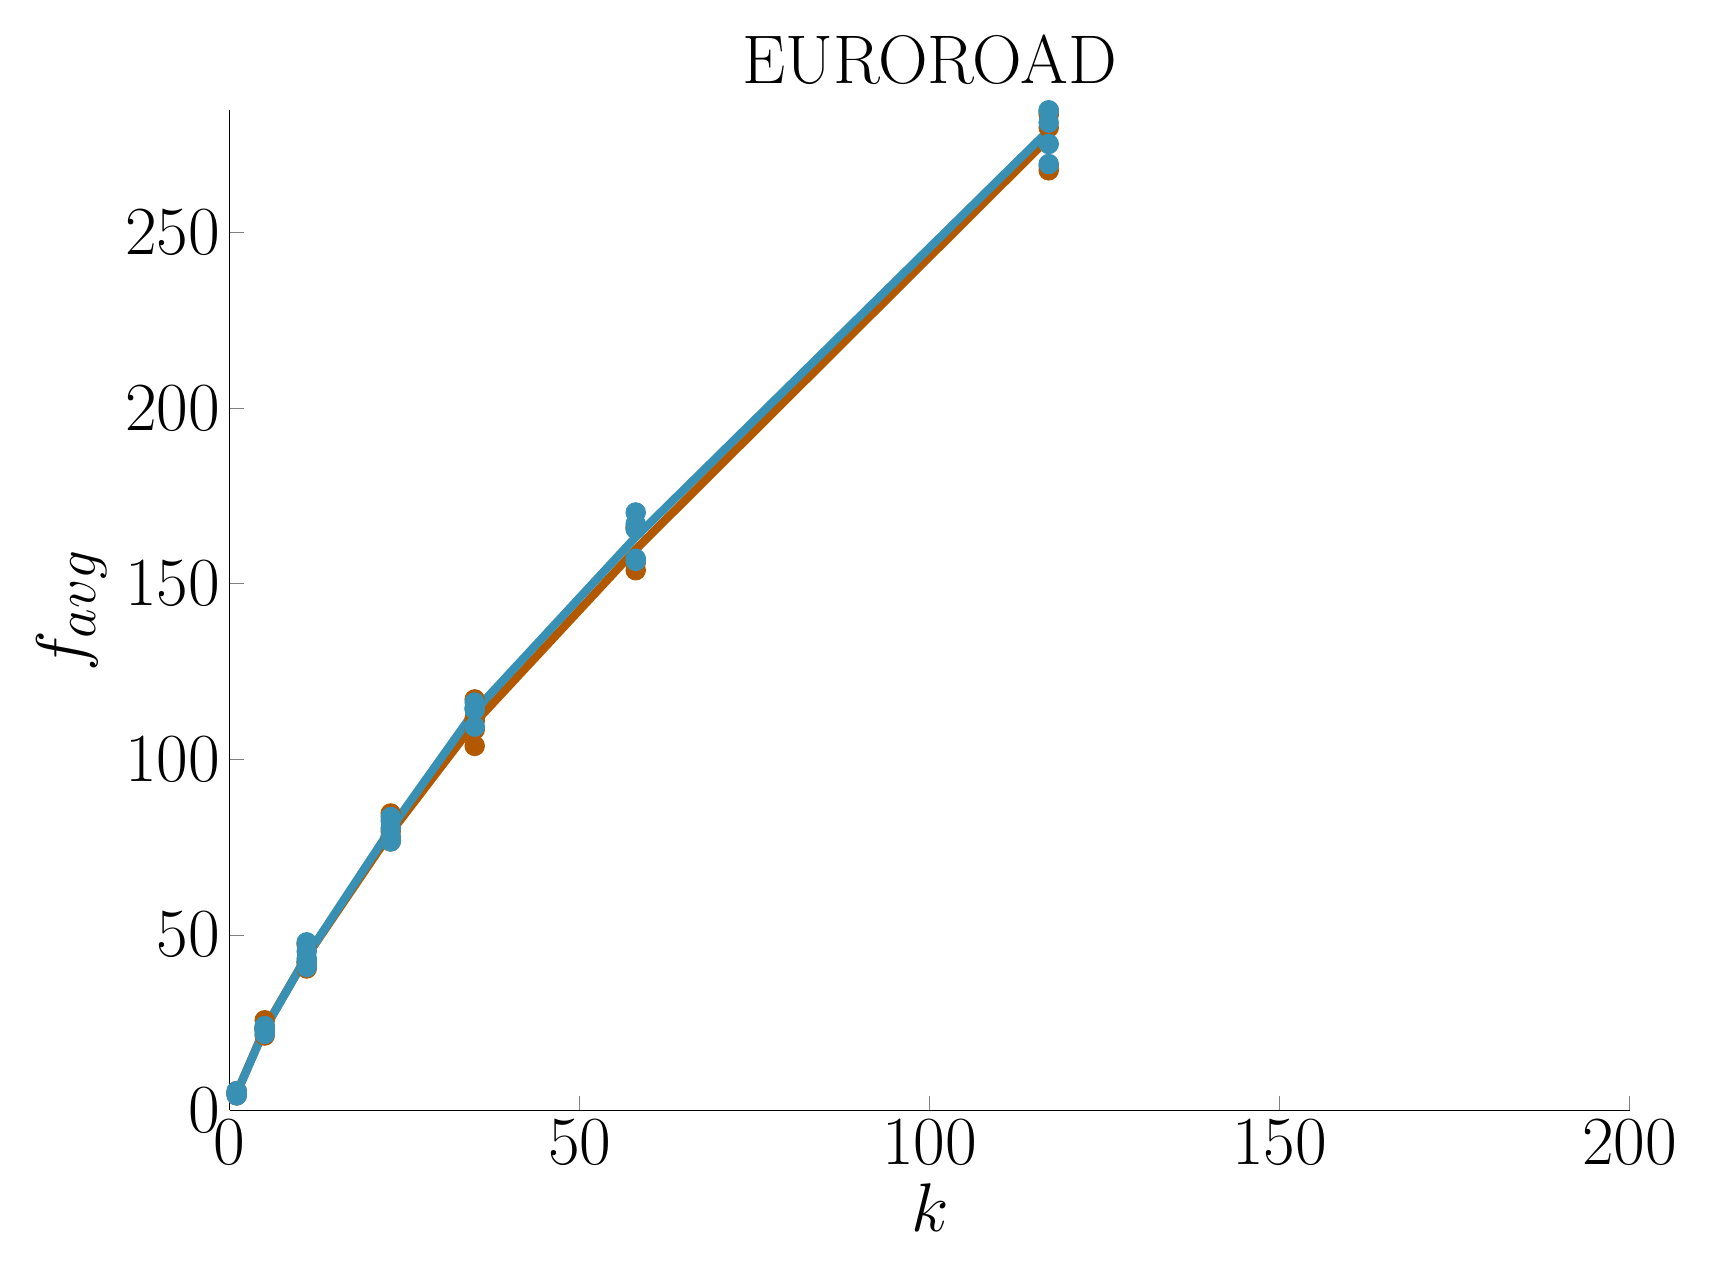
\begin{tikzpicture}

\begin{axis}[%
title style={font=\Huge},
title=EUROROAD,
tick label style={font=\Huge},
label style={font=\Huge},
legend style={font=\Huge},
view={0}{90},
max space between ticks=50pt,
width=7in,
height=5in,
scale only axis,
xmin=0, xmax=200,
xtick={0, 50, 100, 150, 200},
xlabel={$k$},
ymin=0, ymax=284.85,
%ytick={0, 200, 400, 600, 800, 1000},
ylabel={$f_{avg}$},
major tick length=5pt,
axis lines*=left,
legend cell align=left,
clip=false]

\addplot [
only marks,
mark=*,
mark size=3.5pt,
color=orange!70!black,
%solid,
%line width=2pt,
]
coordinates{
(1,4.25)(1,4.8)(1,4.95)(1,4.95)(1,5.45)(5,21.3)(5,23.0)(5,23.0)(5,23.55)(5,25.65)(11,40.4)(11,41.9)(11,42.2)(11,47.1)(11,47.6)(23,76.6)(23,77.05)(23,77.75)(23,79.5)(23,84.55)(35,103.8)(35,108.45)(35,110.95)(35,111.65)(35,117.05)(58,153.85)(58,156.1)(58,156.65)(58,165.95)(58,166.15)(117,267.75)(117,269.0)(117,279.95)(117,283.65)(117,284.35)
};

\addplot [
only marks,
mark=*,
mark size=3.5pt,
color=cyan!70!black,
%solid,
%line width=2pt,
]
coordinates{
(1,4.25)(1,4.8)(1,4.95)(1,4.95)(1,5.45)(5,21.75)(5,22.7)(5,23.35)(5,23.7)(5,24.0)(11,40.8)(11,42.35)(11,43.3)(11,45.3)(11,47.85)(23,76.6)(23,77.95)(23,80.4)(23,82.4)(23,83.55)(35,109.3)(35,114.1)(35,114.45)(35,114.75)(35,116.15)(58,156.5)(58,157.1)(58,165.55)(58,167.05)(58,170.3)(117,269.55)(117,275.25)(117,281.35)(117,284.75)(117,284.85)
};

\addplot [
color=orange!70!black,
solid,
line width=3pt
]
coordinates{
(1,4.88)(5,23.3)(11,43.84)(23,79.09)(35,110.38)(58,159.74)(117,276.94)
};

\addplot [
color=cyan!70!black,
solid,
line width=3pt
]
coordinates{
(1,4.88)(5,23.1)(11,43.92)(23,80.18)(35,113.75)(58,163.3)(117,279.15)
};


\end{axis}
\end{tikzpicture}
\end{document}
